\documentclass[titlepage]{article}
\usepackage[utf8]{inputenc}
\usepackage{lineno, color, graphicx, verbatim, blindtext}
% \linenumbers
% \modulolinenumbers[2]
\usepackage[
backend=biber,
style=numeric,
doi=false,
isbn=false,
url=false,
eprint=false
]{biblatex}
\addbibresource{firstExamRefs.bib}
% \addbibresource{secondaryRefs.bib}
\usepackage{setspace}
\usepackage{tipa}
\usepackage{amsmath}
\usepackage[T1]{fontenc}
% \usepackage{gfsdidot}
\usepackage{venturis}
% \renewcommand{\familydefault}{\sfdefault}

\usepackage{graphicx}
\graphicspath{ {images/} }


\title{Neural Oscillations and the \\ Perception of Spoken Language}
\author{Ivan Iotzov}
\date{September 2018}

\begin{document}

% \fontfamily{cmss}\selectfont
% \fontfamily{lmr}\selectfont
% \fontfamily{phv}\selectfont

\maketitle

%\doublespacing

\section{Introduction} \label{intro}

  Great progress has been made in recent years on the goal
  of decoding the neural computations that undergird 
  human speech processing. This review is intended
  to serve as a brief overview of this work, focusing especially on 
  neural oscillations. I will be examining the role of
  both spontaneous and exogenously driven neural oscillations 
  in speech processing. Although it has been well established that 
  neural oscillations track the amplitude envelope of speech, whether this 
  reflects a bottom-up processing of stimulus acoustics or a top-down 
  speech tracking that is integral to speech comprehension is a matter 
  of ongoing debate. In this introduction I will review
  some basic properties of auditory speech signals, as well as the putative 
  origin and function of various endogenous oscillations that have been 
  measured in the brain. The second 
  chapter will go into more detail on the goals and methods of the auditory 
  processing system in general. The third chapter will be dedicated to 
  discussing the endogenous oscillations in the brain, their interaction with 
  stimulus-driven exogenous oscillations, and the theorized role of these 
  oscillations in speech processing. Lastly, I will attempt
  to integrate all of this information and draw broader conclusions about 
  the functional role of these oscillations in speech processing and avenues 
  for future work that would fill gaps in the literature.

  % First, it is important to delineate the scope of this review. 
  % I will be writing specifically about spoken language processing
  % and so I will attempt to avoid discussion of other, related linguistic topics,
  % such as speech production, reading, etc. 
  % Additionally, I will attempt to limit the discussion below as much as 
  % possible to the processes that parse and then section the incoming auditory 
  % stimulus into usable auditory `objects' \cite{Poeppel2008} that feed into 
  % further lexical and semantic analysis.

  \subsection{Speech Rhythms}

    Spoken language can be roughly categorized as a quasi-periodic, 
    hierarchically organized, sequence of auditory events that encode some 
    information. In \textit{The Speech Chain} \cite{Denes1993}, Peter Denes 
    elegantly laid out the encoding, decoding, and processing that must take 
    place in order for some information to successfully be transferred from one
    person to another in the form of speech (See Fig.\ref{speechChain})

    In this chain (illustrated in Fig.\ref{speechChain}), information
    is transformed in a number of ways when moving from a speaker's intention 
    to a listener's
    understanding. But, for the purposes of this review, it is important to 
    recognize the
    conceptual contribution of treating speech comprehension as a hierarchical 
    process
    that extracts information from an acoustic signal and passes it up a chain 
    of increasing
    complexity until the content of the message is decoded. In this context, 
    we can then move
    to model the stages of the human speech comprehension system as 
    transformations of
    various types on the original speech input signal.

    \begin{figure}
      \centering
      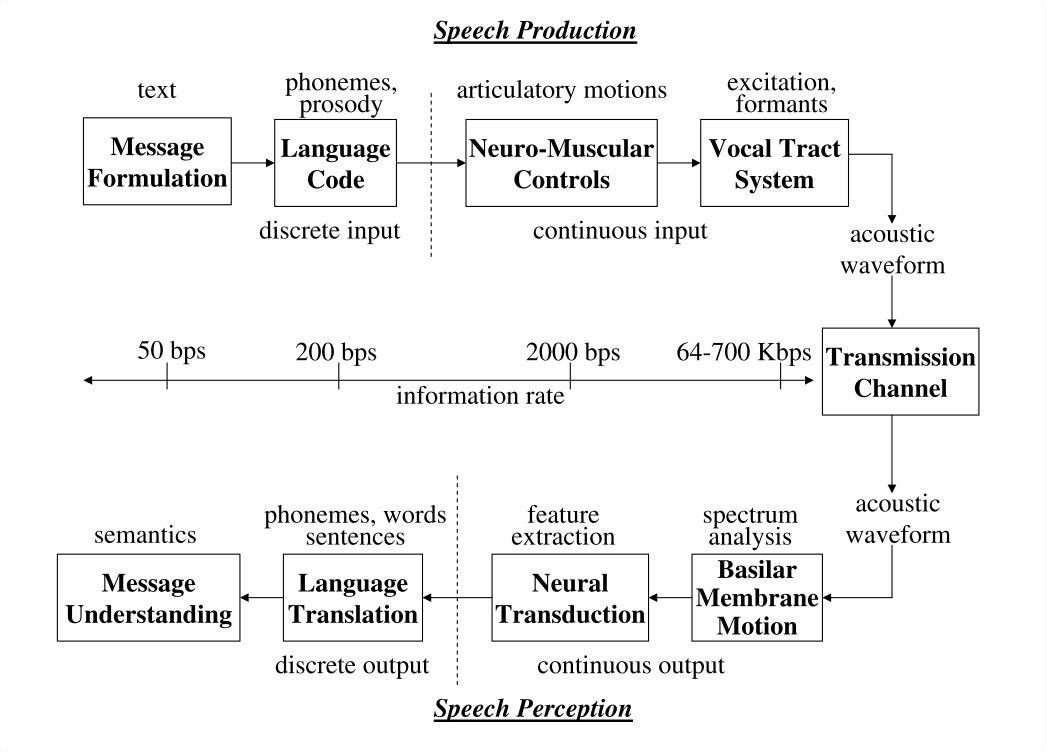
\includegraphics[scale=0.3]{speechChain}
      \caption{The chain of transformations that constitute the `speech chain' as
      described by Denes \cite{Denes1993,Rabiner2007}}
      \label{speechChain}
    \end{figure}

    One of the most fundamental questions in the field is whether language processing
    is accomplished by a general architecture that is also applied to all other sounds
    that are captured by the ear, or whether language has a special set of processing
    rules that apply only to it \cite{Uddin2018}. There is evidence to support both
    conclusions, with some arguing that language is not a special case at all, and all
    of the functions that we see when examining the language faculties in humans can be
    explained by a general, distributed network that is applied an all acoustic analysis
    \cite{Dick2001}. Others see the structure of human language and its uniqueness in the
    animal kingdom \cite{Chomsky1986,Fodor1983} as an indication that there is special
    architecture that supports its use and comprehension. While there is evidence 
    pointing in both directions, there seems to be more suggesting that the faculty 
    of language is indeed special, and that special neural circuits are recruited 
    to facilitate its comprehension \cite{Pinker2005}.

    The breadth and variety of human languages is huge, with
    \textasciitilde 7000 \cite{Simons2017} languages currently spoken across 
    the world. Among these 7000 languages
    there are a large, but consistent number of speech sounds that are produced 
    by humans (see Fig.\ref{ipaChart}). One of the primary challenges of both
    linguists and neuroscientists working in the area of speech processing is
    how the human brain is capable of dealing with information that comes in 
    such a diverse array of languages, each with their own lexical, semantic, 
    and stylistic rules.

    Despite all this variation, every human language is intelligible to those 
    that speak it. Indeed, the ability to learn languages outside of one's 
    native language points to the universality of the mechanisms on which 
    speech comprehension is built. In the case of speech, modulations less than 
    16 Hz, with a notable peak at 3-5 Hz, are the basis for the syllabic rhythm 
    \cite{Giraud2012,Greenberg2003}.

    One way to characterize these rhythms is through analysis of the 
    modulation spectrum of speech. The modulation spectrum is defined as 
    `the spectrum of the temporal envelope of sound and
    reflects how fast sound intensity fluctuates over time' \cite{Ding2017}. 
    In a study of
    a large audio corpus of 9 languages, Ding et al. \cite{Ding2017} found a 
    remarkably
    consistent peak for the modulation spectrum of spoken language at 2-10 Hz, 
    with a particular
    peak at \textasciitilde 5 Hz. This same 5Hz rate has also been found in 
    empirical studies of syllabic
    rate in a number of languages \cite{Pellegrino2011} and seems to be a 
    consistent, intrinsic
    property of speech, regardless of the language that is being spoken.

    These temporal modulations are likely important to the processing of 
    spoken language as they provide consistent acoustic landmarks for the 
    chunking of incoming acoustic signals into discrete units that can then be 
    decoded. Examination of the modulation spectrum has not been the only 
    method of measuring the rhythmic 
    aspects of speech. There is a rich literature in the field of linguistics 
    dealing with how and on what basis different languages are arranged in time.
    In this system of classification that has been developed, languages can be 
    stress-timed or syllable-timed \cite{Nakatani1981,Dauer1983}. Stress-timed 
    languages (such as English or Dutch) rely on a series of stressed or 
    un-stressed syllables to generate the rhythm that is perceived in speech. 
    Syllable-timed languages (such as French) rely only on the timing of the 
    syllables themselves, and not on the stresses that are placed on them. Note
    that Japanese has been placed in a class of its own, said to have a unique 
    mora based timing scheme.

    This effort by linguists to classify languages into different timing 
    schemes is primarily an effort to force the quasi-periodic rhythm of human 
    speech into a more isochronous form. If there is an underlying isochronicity
    below the relatively messy rhythms that are present in natural language, 
    then there is a relatively easy way to describe how humans can perceive 
    speech that is independent of language and can also be easily compared to 
    the perception of musical rhythms which are fundamentally based in their 
    isochronicity. 

    This paradigm has been challenged in a number of ways 
    \cite{Ramus2000,Grabe2002}, with critics primarily pointing to the 
    subjective and often contradictory classification of languages that can 
    change based on the corpus of speech used and the judgments of the 
    observer. The problem of classification in this paradigm has led some 
    to focus solely on stress timing as a rhythmic framework in all languages 
    \cite{Hayes198433,Martin1972}. This framework also has some empirical 
    justification as several ERP studies have found that the brain can detect 
    violations of expected stress patterns 
    \cite{Rothermich2012,Knaus2007,Haegens2018}.
    
    \subsubsection{Classes of Phonemes}

    Phonemes can either be classified by their acoustic properties,
    or by the mode of their generation in natural human speech. In the latter
    method, they are typically divided into stops, nasals, fricatives, 
    laterals, rhotics,
    clicks, and vowels \cite{Ladefoged1996}. Though, no language makes use of 
    every speech sound
    that can be produced by the human vocal tract, and some sounds are found 
    much
    more rarely than others. These distinctions are far more useful for the 
    linguistic analysis
    of speech than they are for the acoustic analysis, so we turn to the main 
    acoustic
    differentiation of speech sounds: periodic, voiced speech versus aperiodic, 
    unvoiced speech.
    The difference between these two can be clearly seen from both their 
    waveforms, as well as
    their frequency domain spectra (See Fig.\ref{exampleSpectrogram}).


    \begin{figure}
      \centering
      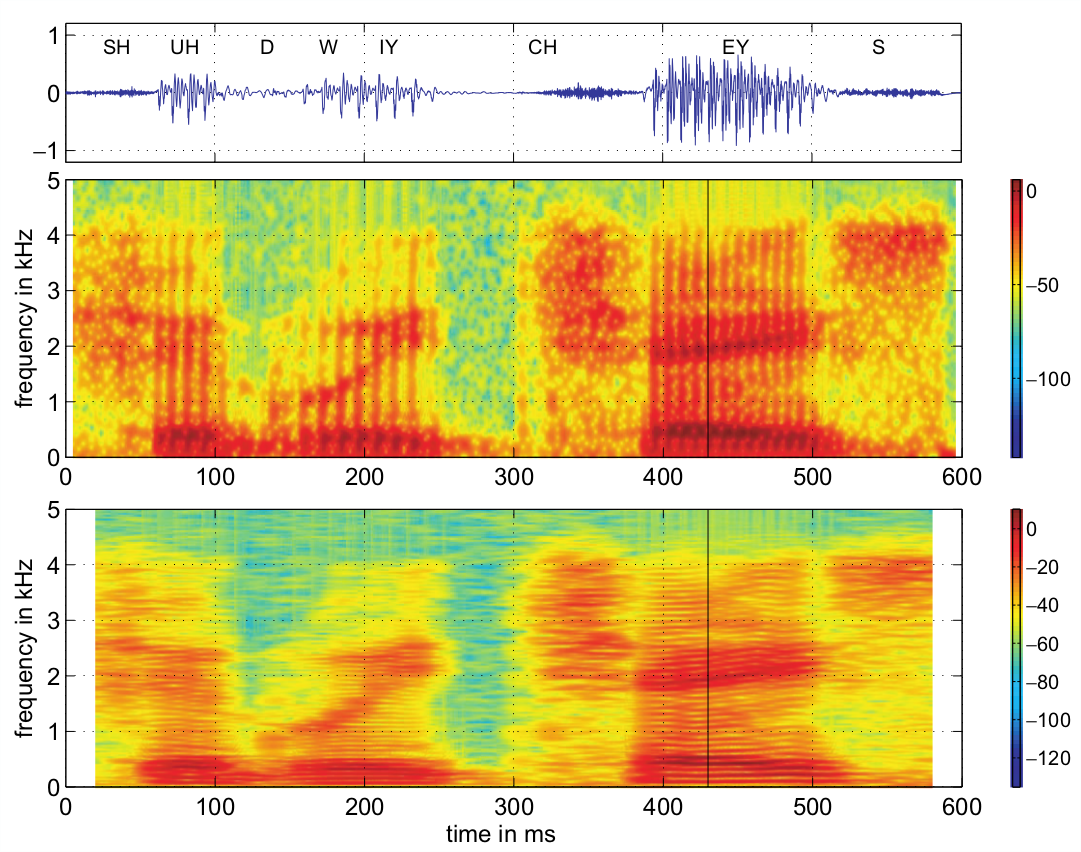
\includegraphics[scale=0.23]{exampleSpectrogram}
      \caption{Waveform and 3D Spectrogram of the phrase `Should we chase' \cite{Rabiner2007}}
      \label{exampleSpectrogram}
    \end{figure}


    The differences between these two classes of speech sounds is explained
    through differences in their modes of production. For instance, the unvoiced
    fricative \textipa{[S]} (the first syllable in Fig.\ref{exampleSpectrogram})
    looks like random noise, while the voiced vowel \textipa{[U]} appears to have
    a definite structure with periodic features. This is because \textipa{[S]} is
    produced by the constriction of airflow out of the mouth through use of the tongue,
    while \textipa{[U]} is produced by the modification of vibrations generated in the
    vocal cords. The fact that voiced sounds are generated by vocal cord vibrations gives
    them a special structure that makes them much easier to identify in the context of
    feature extraction, and makes them important markers in computer speech recognition
    \cite{Gutierrez-Osuna2017}.

    How the brain parses differences between different types of phonemes, particularly
    those that lack discernable spectral content (such as fricatives) is still an area
    of active study. The ability to discern between meaningless noise and a meaningful
    phoneme must rely on information outside of just the spectral content of the
    speech signal itself, as the two might be indistinguishable based on just this information.
    Instead, it is likely that timing and rhythm play an important role in the differentiation
    of speech sounds. The order and precise timing of the delivery of a speech sound has a
    strong effect on how it is perceived and these context effects have strong influences on
    the human perception of speech and language.


    \begin{figure}
      \centering
      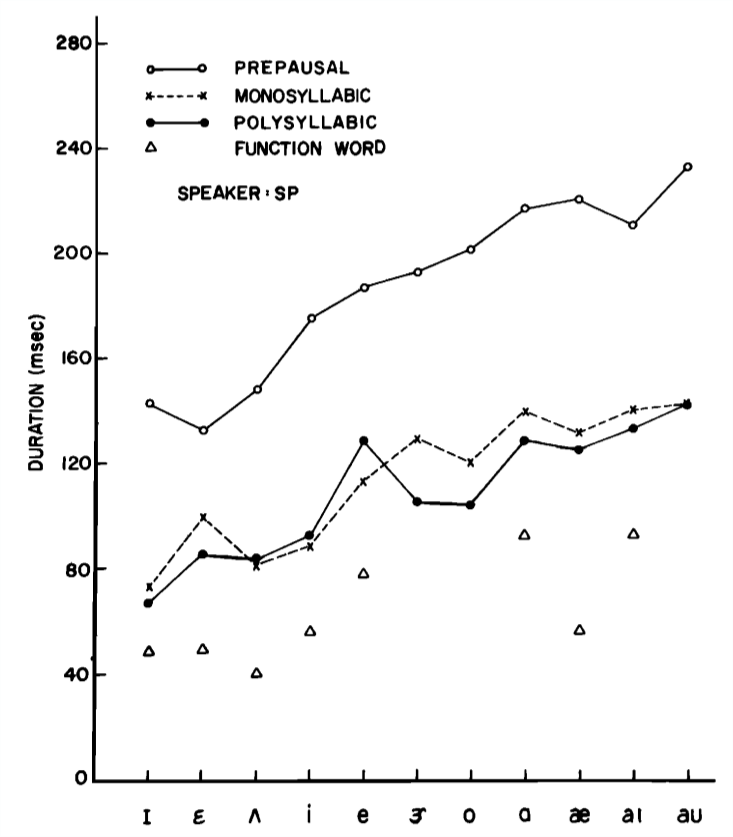
\includegraphics[scale=0.3]{vowelDuration}
      \caption{Average duration of a selection of vowels under three different
      speaking conditions from one speaker \cite{Umeda1975}}
      \label{vowelDuration}
    \end{figure}

  \subsubsection{Speech Formants}

    An important feature of voiced speech sounds that seems to be critical 
    in their
    recognition are the formants of the vowel sound. Formants are defined as 
    being distinctive
    frequency components of a speech signal that are generated by the resonance
    of the human vocal tract \cite{Denes1993}. They can be seen clearly in the 
    speech spectrogram
    (See Fig. \ref{formants}) as areas of particularly high energy within a 
    certain frequency band.
    Formants come about due to the resonance of the vocal tract. By moving 
    the articulators
    (lips, tongue, etc.), the size and shape of the cavities in the vocal tract 
    are altered and
    therefore so are the resonant frequencies. All vowel sounds are produced 
    through this manipulation
    of the resonant frequencies of the vocal tract which gives them a 
    characteristic, periodic
    structure that can be readily identified.


    By convention, vowel formants are assigned numbers in order of ascending 
    frequency. So, the
    lowest frequency formant of a vowel is assigned $F_1$, the next lowest 
    $F_2$, and so on.
    Many vowels can be distinguished from one another simply by the use of 
    these first
    two formants \cite{Schnupp2011}, making them important markers in both 
    human and computer
    speech recognition. For example, the vowels in Fig.\ref{formants} can 
    be differentiated
    from one another simply by reference to their $F_1$ and $F_2$ frequencies. 
    The importance
    of these formants to biological auditory comprehension was demonstrated 
    in part by
    Young and Sachs (1979) \cite{Young1979}, who showed that auditory nerve 
    discharges in
    response to auditory stimuli reflect the formants when vowels are presented.


    \begin{figure}
      \centering
      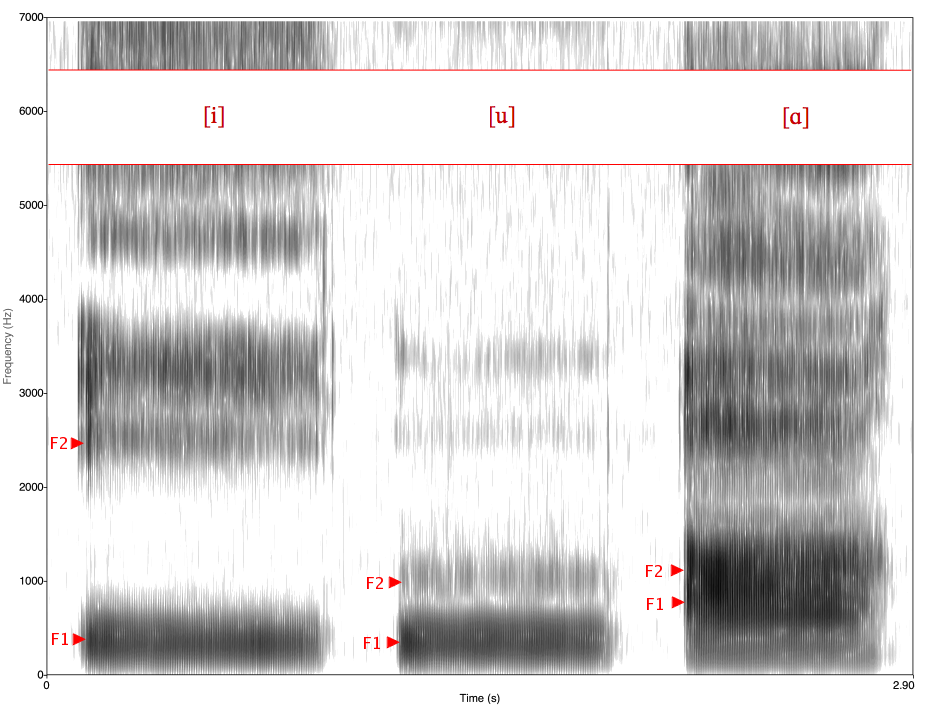
\includegraphics[scale=1.6]{formants}
      \caption{Spectrogram of a native speaker of American English
      pronouncing the vowels \textipa{[i, u, A]} \cite{pict}.}
      \label{formants}
    \end{figure}

  \subsection{Endogenous Brain Rhythms} \label{endogenousBrainRhythms}

    There exist a number of neural rhythms that are innately present in the
    human brain. Roughly speaking, these are divided into $\alpha$ (8 - 12 Hz),
    $\beta$ (12 - 30 Hz), $\theta$ (4 - 8 Hz), $\delta$ (1 - 4 Hz), $\gamma$
    (30 - 80 Hz), and high $\gamma$ (80 - 150 Hz)
    \cite{Muresan2008,Rangaswamy2002}. These are roughly divided by the
    frequency of the oscillations and their suspected behavioral correlates.
    There is clearly overlap between these categorizations and it is difficult
    to make very clear distinctions between the various classes of neural
    oscillations. Despite this, there are some clear behavioral correlates in
    each of these frequency bands, and there have been attempts to localize the
    neural circuits responsible for their generation \cite{Michel1992}.

    Some of these rhythms are particularly relevant for the study of speech
    processing as they appear to have the same frequency as the typical speech
    rhythm and their power in EEG signals increases as a function of
    intelligibility. Particularly important to speech processing appear to be
    the $\delta$, $\gamma$, and $\theta$ rhythms \cite{Ghitza2009,Meyer2018}.
    In the case of the $\theta$ rhythm, Oded Ghitza has been a particularly
    strong advocate for the idea that the $\theta$ rhythm is crucial to parsing
    the speech signal into syllabic chunks which are the fundamental unit of
    speech processing. He refers to this fundamental unit as the
    `theta-syllable' \cite{Ghitza2013a} and claims that it is central to the
    theory of speech comprehension as a faculty facilitated by cortical
    entrainment to speech signals. In this view, the theta-syllable is defined
    as `a theta-cycle long speech segment located between two successive vocalic
    nuclei'. A vocalic nucleus is the critical section of a syllable (often a
    vowel) that can be preceded or followed by other marginal sounds (often
    consonants). For example, the word \textit{window} can be divided into the
    syllables \textipa{/"wIn/} and \textipa{/doU/}. In the \textipa{/"wIn/}
    syllable, the \textipa{/I/} sound functions as the nucleus while the
    \textipa{/w/} and \textipa{/n/} sounds are on the margins of that nucleus.

    In this interpretation, the theta rhythm is essentially the `master' rhythm
    that is responsible for the main chunking of the incoming speech stimulus
    and leads to the efficient parsing of syllables. This is crucial to
    understanding speech comprehension because of one of the most important
    mysteries in this area is how the brain chunks information into syllables
    that can then be parsed and transformed into higher-order representations.
    Without the ability to transform incoming acoustic information into smaller
    `chunks', the brain would have no ability to separate out syllabic
    information and parse what the speech information in a given chunk of time
    is. Instead, it would appear more as an undifferentiated mass.

\section{Neural Auditory Processing} \label{corticalAuditoryProcessing}

  In the above sections, the emphasis has been on the properties of the
  acoustic stimulus itself, its important features, and the mechanisms by
  which it is detected by the human auditory system. This chapter is dedicated
  to the transformation and integration of that acoustic information after it
  has been detected by the auditory system. Once an acoustic stimulus has
  been transformed into neural impulses by the machinery of the inner and outer
  ear, it proceeds through the brainstem and into the cortex. Roughly,
  information travels from the cochlea to the cochlear nuclei of the brainstem,
  the superior olive, the inferior colliculus, the medial geniculate nucleus of
  the thalamus, and finally to the primary auditory cortex
  \cite{Hickok2007,Webster1992}. This outline of the auditory pathway is
  a gross oversimplification but useful for this review as it shows that 
  there is some processing of incoming speech signals being done before the
  neural impulse reaches the brain. Brainstem and subcortical innervation
  sites are more numerous than described above, and there are also significant
  efferent connections from the higher auditory processing areas all the way
  down to the cochlear neurons themselves \cite{Kandel2000,Webster1992}. This
  overview is meant to provide a rough sketch to demonstrate the hierarchical
  and interconnected nature of the auditory processing pathways as well as to
  give a general view of how information proceeds from the ear to the cortex.
  Here, we will mainly concern ourselves with the processing of neural signals
  once they reach the primary auditory cortex and other related areas.


  This pathway shares some features of the visual processing pathway. It is
  hierarchical, but not strictly so, and it contains significant
  back-projections and divergent pathways \cite{Webster1992,Hickok2007}.
  Hickok and Poeppel, two prominent voices in the field, maintain that there
  are actually two parallel cortical pathways for acoustic information much
  like the parallel processing pathways found in the visual system
  \cite{Hickok2007,Hickok2004,Hickok2000}. The ventral auditory processing
  stream is thought to underlie the conversion from acoustic signals into
  lexical and semantic representations. The analogy could be drawn to the
  ventral visual stream, which is thought to mainly be responsible for visual
  object recognition. In a similar way, the ventral auditory stream underlies
  the ability to recognize acoustic `objects' and connect those to phonological
  or semantic meanings \cite{Parker2005,Rauschecker2009}. The dorsal stream of
  the auditory pathway has a less well-understood function, but it is thought
  to be involved in sensorimotor integration in much the same way as the dorsal
  visual stream is. In particular, Hickok and Poeppel theorize that this
  network is crucial in the development of speech as it integrates the sounds
  that are perceived and facilitates the motor learning task of learning to
  speak.

  A competing theory put forward by Angela Friederici \cite{Friederici2011} is
  that there are actually two ventral pathways and two parallel dorsal pathways.
  In this theory, there is one ventral pathway from roughly Brodmann's area 45
  to the temporal cortex and another from the frontal operculum (FOP) to the
  uncinate fascile (UF). These two ventral pathways are hypothesized to mainly
  be responsible for language processing and the processing of adjacent elements
  in an audio signal. The two dorsal pathways are thought to connect from the
  temporal cortex to the premotor cortex, as well as from the temporal cortex
  to Brodmann's area 44. The first pathway is thought to mainly support
  auditory motor functions similar to those proposed by Hickok and Poeppel,
  while the second is thought to be involved in more high-level language
  processing functions. Specifically, the second pathway is thought to provide
  a complement to the ventral streams in that it connects information that
  is not adjacent in the auditory stream and allows for grammatical analysis
  and connections.

  \subsection{Primary Auditory Cortex} \label{primaryAuditoryCortex}

    \begin{figure}
      \centering
      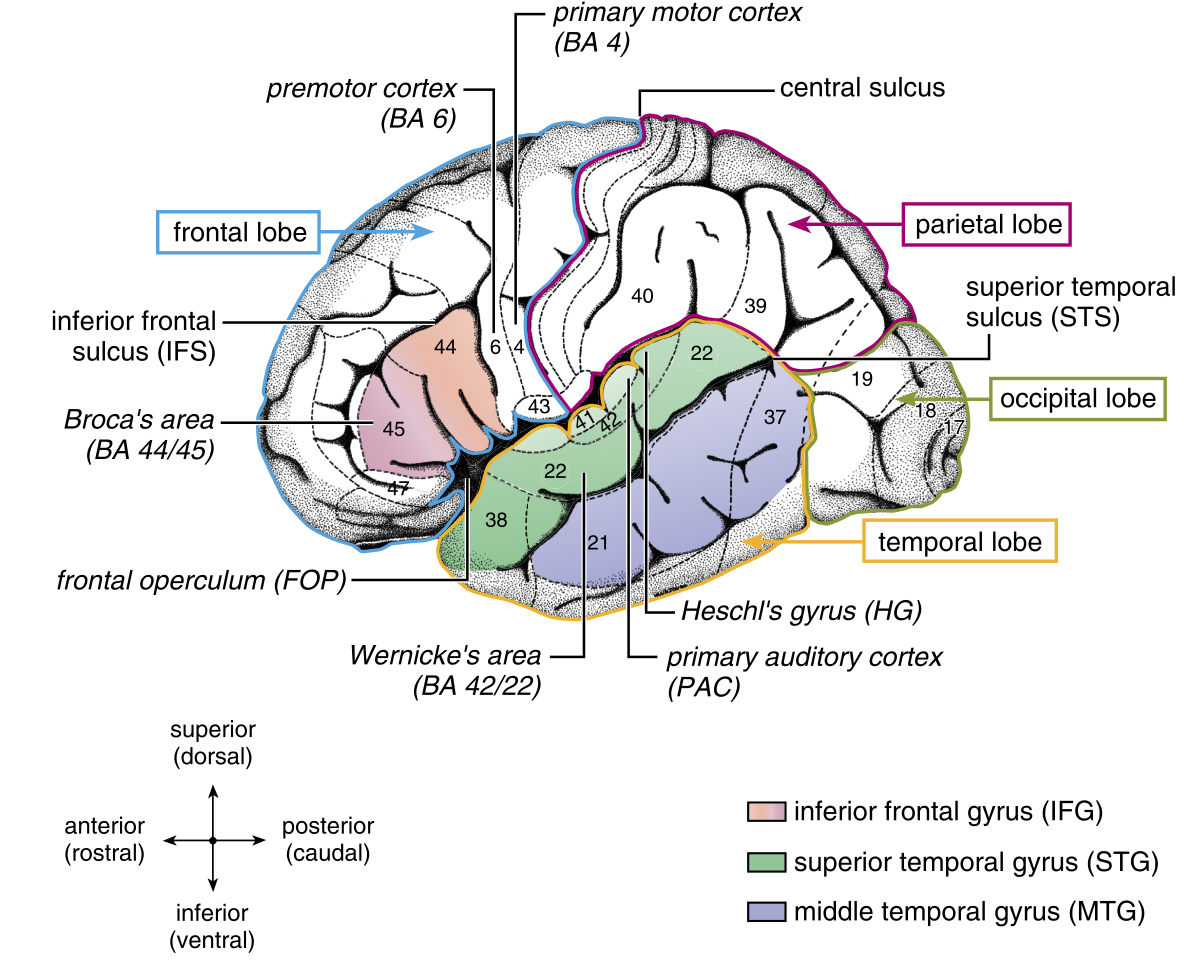
\includegraphics[scale=0.25]{primaryAuditoryAnatomy}
      \caption{This figure shows the gross anatomy of the left hemisphere
      of the human brain. The lobes, Brodmann's areas, and other areas
      of interest have been highlighted. \cite{Friederici2011}}
      \label{primaryAuditoryAnatomy}
    \end{figure}

    The primary auditory cortex (A1) is the main target of auditory information
    from the sensory neurons in the cochlea and is the backbone of auditory
    perception. It is located on the superior temporal gyrus
    (see Fig. \ref{primaryAuditoryAnatomy}) and can be divided into a primary
    area and various belt or peripheral areas \cite{Purves2001}. A1 is organized
    tonotopically, meaning that there is a separation by frequency of the
    incoming auditory signals, and that neighboring neurons respond to
    neighboring frequencies \cite{Lauter1985}. Organization of A1 is analogous
    to the topographical mapping that can be found in V1, and mirrors the
    tonotopic organization of the basilar membrane, discussed above.
    Therefore, A1 can be said to
    have a frequency `axis', groupings of neurons that react selectively to the
    frequency content of incoming auditory signals. Additionally, A1 contains an
    orthogonal `axis' that processes information related to the binaural aspects
    of incoming auditory signals and may serve localization or source
    identification purposes \cite{Purves2001}.


    Bilateral destruction of A1 results in cortical deafness, resulting in a
    total loss of hearing faculties in those affected. In order to manifest,
    this disorder requires total bilateral destruction of A1. Due to this, as
    well as the relatively high degree of redundancy in subcortical auditory
    structures, the disorder is quite rare \cite{Polster1998}. Additionally,
    subcortical processing of auditory signals may preserve some auditory
    capacities even in patients with this condition \cite{Cavinato2012}. More
    commonly, following damage to the cortical auditory areas are the conditions
    of auditory agnosia, pure word deafness, and phonoagnosia.

    Auditory agnosia
    is a condition in which patients are incapable of identifying sounds such
    as coughing or whistling, but show no evidence of impaired auditory speech
    comprehension. Pure word deafness is essentially the opposite of auditory
    agnosia, where patients are incapable of comprehending speech while
    maintaining their ability to speak, read, and identify sounds.
    Interestingly, some patients with pure word deafness retain their ability
    to extract information about a speaker (such as age, sex, etc.) based on
    their speech \cite{Polster1998}. Phonoagnosia is a condition analogous to
    prosopagnosia (inability to recognize familiar faces), where patients
    lack the ability to recognize familiar voices.


    These conditions provide insights into the different functions that are
    performed by the auditory processing system and demonstrate that these
    functions can be dissociated without disrupting the system completely. This
    observation points to the fact that the human auditory system is attempting
    to extract multiple types of information from an incoming auditory signal
    and that the methods for extracting this information involve separate
    cortical processing mechanisms.


\section{Neural Entrainment \& Stimulus-Driven Dynamics} \label{entrainment}

  Entrainment is defined as the synchronization of two or more oscillators 
  that can generate their own rhythms in the absence of any rhythmic input. In
  the cases that will be discussed below, the oscillators are a neural 
  population, and a rhythmic input stimulus (i.e. speech). This definition is 
  intended to contrast the frequency and phase entrainment responses with 
  others, such as the envelope-following response.

  \subsection{Brainstem Entrainment} \label{brainstemEntrainment}

    The Auditory Brainstem Response (ABR) is a well-known neural response to
    auditory stimuli that was discovered more than 40 years ago
    \cite{Jewett1971,Jewett1970} and has seen widespread use in clinical
    settings for determining auditory thresholds or diagnosing neuropathologies
    \cite{Skoe2010} and is especially popular for hearing screening in infants.
    Measurement of this response is one of the most common clinical applications
    of auditory evoked potentials and the typical waveform is well
    characterized.

    The test typically consists of presenting a subject with a series of click
    stimuli while recording neural activity through surface electrodes placed on
    the scalp. The averaged activity is then examined for the characteristic
    response that develops over a window of \textasciitilde 10ms and consists
    of a series of waveform peaks labeled \textit{I-VII}
    \cite{Sininger1993,Bhattacharyya2017}. This activity is a stimulus-driven
    response that is generated in the brainstem and the auditory nerve and as
    such cannot be equated with the conscious perception of a stimulus, but
    does seem to be highly predictive of a subject's level of hearing loss
    \cite{Sininger1993}.

    More recently, there has been work involving the measurement of the ABR in
    response to complex stimuli, as opposed to the simple clicks or tones that
    were used previously. For example, Galbraith et al. (1995)
    \cite{Galbraith1995} found that intelligible speech could be recovered from
    the ABR that is recorded while the subject is presented with speech stimuli.
    Further studies have been conducted looking at a diverse range of stimuli
    including words, phrases, and music, and this work is ongoing. ABR still 
    remains a reliable indicator of healthy auditory processing precisely 
    because it is a more low level response that is easily disrupted by problems
    at the level of the ear or afferent auditory fibers.

    However, due to the low-level nature of the ABR, it is not a very useful 
    response for studying the higher-level auditory responses, such as speech 
    processing. The fact that it responds mainly to changes that occur at the 
    level of the ear limits its usefulness in studying cortical processing of 
    auditory input.

  \subsection{Cortical Entrainment and Envelope Following} \label{corticalEntrainment}

    In addition to entrainment occurring in the brainstem, it is also possible
    to measure cortical entrainment in response to acoustic stimuli with methods
    such as electroencephalography and magnetoencephalography. This type of
    entrainment typically has the best correspondence to the temporal
    modulation of the amplitude envelope of the speech signal
    \cite{Ding2014a,Ding2014,Nourski2009,Horton2014}. This cortical entrainment
    seems to be linked to a number of behavioral factors, such as attention
    \cite{Dmochowski2016,ZionGolumbic2013} as well as engagement with the
    stimulus \cite{Dmochowski2017}. This entrainment is clearly an exogenous,
    stimulus-driven process, which is illustrated by the consistent responses
    elicited across subjects by the same audio or visual stimuli
    \cite{Cohen2017,Petroni2017}.

    In discussing neural entrainment to any feature in natural speech, it is 
    important to recall that speech is hierarchically structured and therefore 
    the auditory stream is encoding information at different rates. For example,
    the syllabic rate of a certain speech segment may be 4Hz, but this is 
    concurrent with a phrasal rate of, say, 2Hz. Even if the 4Hz rhythm is the 
    only one that is `actually' contained within the stimulus, there should 
    still be a response in the brain to the 2Hz phrasal rhythm in order for 
    us to be able to comprehend the speech. This phenomenon has been demonstrated
    empirically \cite{Ding2015} and corresponds with the idea that the brain is
    tracking rhythmic properties of acoustic stimuli. 

    It has been demonstrated that cortical neurons entrain to the amplitude
    oscillations present in speech stimuli, but the causal mechanism of this
    entrainment is still being debated in the field. Some claim that it is
    caused by entrainment to low-level features of speech sounds 
    (defined as the sound amplitude and spectral content), basically a
    version of an auditory steady-state potential (such as those found in the
    brainstem discussed in section \ref{brainstemEntrainment}). Others
    maintain that this phase entrainment is a product of more
    high-level speech sound features and reflects a processing of information
    carried in the speech signal by the brain.

    Zoefel and VanRullen \cite{Zoefel2016} address this question by presenting
    subjects with mixed speech/noise stimuli that retain the patterns of
    higher-level features, but do not have the fluctuations in spectral content
    and sound amplitude that some claim is the basis for the phase entrainment
    response. They found that neural phase entrainment occurs despite the
    missing low-level content, indicating that it is the higher-level features
    that drive this response. Additionally, they find that reversing their
    speech/noise mixture stimuli does not eliminate the phase entrainment
    response. This finding seems to indicate that the entrainment is in
    response to higher-level features, but only those that are acoustic in
    nature and not linguistic features, as those are absent in time-reversed
    speech.

    What, exactly, the functional role of this entrainment to the speech
    envelope is remains a topic of debate in the field, but there has recently
    been strong evidence to support the hypothesis that cortical entrainment to
    the speech envelope facilitates comprehension of the speech signal
    \cite{Ding2014a,Ding2012,OSullivan2015}. These observations do show that 
    there is a link between speech intelligibility and stronger neural 
    entrainment, but it is not possible to tell what the precise cause is. It 
    could be due to a stronger evoked response to a stimulus that is easier to 
    hear and understand. Or, it could be due to stronger recruitment of the 
    oscillatory mechanisms that facilitate the intelligibility of the speech.

    Some studies have looked to address this problem by dissociating these 
    two possible mechanisms of neural entrainment. One by K{\"o}sem et al.
    \cite{Kosem2017} attempted to do this by quickly changing the speech 
    rate at the end of a sentence. If the observed neural entrainment to the 
    stimulus is indeed caused by internal oscillatory mechanics, then these 
    oscillators would entrain to the initial part of the sentence and when the 
    speech rate is changed at the end of the sentence, it will be mis-perceived.
    This is indeed what they found. Participants were asked to indicate whether 
    they heard a short \textipa{[A]} or a long \textipa{[a:]} at the end of the 
    sentence, and their answer was dependent on whether the speech preceding 
    this vowel was presented at a fast or a slow rate. This study points to the 
    fact that neural entrainment does not simply reflect an evoked response 
    to low level features of the speech input, but an endogenous, ongoing 
    neural process of speech parsing that influences our perception. 

    The fact that cortical neurons track the amplitude envelope of speech
    signals is now well-known and is considered an important part of the speech
    processing pathway. But, the interaction between natural cortical rhythms
    (discussed in Section \ref{endogenousBrainRhythms}) and the envelope following
    response is still not completely understood, and its functional role remains
    a subject of debate. There is abundant evidence that broad-spectrum EEG
    signals can be used to decode which speaker is being attended to by a
    subject in a cocktail party scenario \cite{Horton2014,DeTaillez2018}, but
    these studies only offer a partial picture of the role of cortical
    envelope-following responses in speech comprehension.

    For instance, Zion Golumbic et al. \cite{ZionGolumbic2013} were able to
    localize the envelope tracking response both in terms of cortical location
    as well as which frequency band was recruited for entrainment using
    electrocorticography (ECoG) in a cocktail party scenario with two speakers.
    They found found that there is a significant ability to predict which
    speaker is being attended in two different frequency bands that they term
    `low-frequency' (1-7 Hz) and `high gamma' (70-150 Hz). Further, they found
    that cortical locations in which these two frequency bands possessed
    significant predictive power differed. Both showed a very strong response
    in the superior temporal gyrus, which is to be expected given that is the
    location of the early cortical auditory areas, but the high gamma band
    showed a more widespread distribution around the brain, while the
    low-frequency band was more concentrated in frontal and temporal areas.

    These findings point to the conclusion that the envelope following response
    is not monolithic, and that there are multiple functional roles filled by
    the envelope following response.

    One of the most popular theories currently is that speech signals are
    essentially a quasi-rhythmic input which certain innate cortical rhythms are
    recruited to track. This tracking then enables both the exclusion of
    irrelevant speech signals \cite{Horton2014,OSullivan2015} as well as the
    syllabic parsing that is thought to be accomplished by the innate theta
    oscillations in the cortex \cite{Doelling2014,Ghitza2013b}.

    Interestingly, speech remains intelligible despite a large amount of
    information in the speech signal being destroyed. Speech information is
    resistant to both degradation of temporal as well as spectral information
    \cite{Silipo1999,Drullman1994}. Barring total elimination of temporal and
    spectral information, it is only when both are sufficiently degraded that
    speech becomes unintelligible \cite{Elliott2009}. Related to this, the
    phenomenon of speaker gender identification is also reliant on similar
    information and can be modulated by changing the information present in the
    temporal and the spectral domain. Elliott and Theunissen \cite{Elliott2009}
    found that speaker gender identification rate can be significantly
    degraded by removing spectral modulations between 3 and 7 cycles/Hz and that
    this specifically reduced the subjects' ability to correctly identify
    female speakers. They postulated that this is because the female vocal
    spectrum has more power in this specific range and this is what
    contributes to `sounding like' a female speaker. Clearly, there is more
    information than just that necessary for comprehension that is embedded
    in the temporal and spectral modulations of speech and it is important to
    parse out what is necessary for the comprehension of speech and what
    information is supplemental, but not necessary to the bare comprehension
    of speech.

    This brings up a large controversy in this field of study, which is the
    question of whether neural entrainment occurs because of the recruitment of
    natural neural rhythms that are simply used for alignment and parsing of the
    incoming speech signal, or whether these oscillations are actually
    generated by the speech signal itself and do not rely on oscillatory
    activity that is always ongoing in the cortex. This distinction is
    important because it colors how the increase in stimulus-aligned activity
    is interpreted. In the case of innate, ongoing oscillations being recruited
    to speech comprehension purposes, the activity that is elicited by
    presentation of a stimulus is used in `chunking' the incoming speech signal
    into segments that can be processed for lexical information and then
    combined to give some type of semantic meaning to a sentence. On the other
    hand, if the increase in stimulus-aligned activity is due to the
    emergence of a signal in the brain that tracks the amplitude envelope of
    the incoming speech signal, then it would seem that the analysis being
    performed in the brain is not of the `chunking' type, but involves
    synchronizing to the rate of the incoming speech signal and using
    information other than the relation of the incoming speech signal to
    innate oscillatory activity to process and comprehend speech.

  \subsection{Effects of Visual Information on Entrainment}

    Though this review is focused on the processing of auditory information, it
    is worth taking time to discuss the contributions of other modalities to
    the auditory comprehension process and how those other modalities might
    influence the neural signals that we can measure. Auditory information,
    especially in the case of speech, is rarely present without any visual
    input. When we are speaking with another individual, that person's facial
    expressions, lip movements, and body language all influence the our
    understanding of their speech. Especially in the case of speech that is
    difficult to hear or ambiguous, visual cues provide significant information
    that guides the comprehension of the auditory signal.

    For instance, it is well documented that, especially under noisy
    conditions, being able to see a speaker's face contributes significantly to
    the ability to understand that speaker \cite{Sumby1954,Erber1969}.

  \subsection{Comprehension Effects of Entrainment}

    In recent years, there has been a growing body of literature that supports
    the hypothesis that cortical entrainment to the temporal modulation of
    speech is the critical process that enables speech comprehension
    \cite{Meyer2018,Morillon2015,ZionGolumbic2013,Doelling2014}. This
    entrainment is found in both frequency (FM) and amplitude (AM) modulation,
    though the two are not independent \cite{Ding2009}. Ding \& Simon (2009)
    \cite{Ding2009} find that for a signal that is both frequency
    ($f_{FM}=40Hz$) and amplitude ($f_{AM}\leq 15Hz$) modulated, there is an
    auditory steady-state response at both $f_{FM}$ as well as at $f_{AM}$ but
    that the response at $f_{FM}$ is amplitude and frequency modulated with
    fundamental frequency $f_{AM}$. This points to the fact that when we speak
    about entrainment of signals in the brain there are multiple different
    `sites' of entrainment and that neural oscillations can be entrained to
    multiple features of a stimulus.


\section{Conclusion}

    In this review, I have laid out the background and basis for 
    various theories for the role of oscillatory mechanics in speech 
    comprehension. I have gone over the various properties of spoken language 
    that are used by the brain in order to decode the information present in 
    speech, as well as some of the basic and fundamental processes that 
    speech information undergoes as part of the speech comprehension process. 
    Most importantly, I have looked to 

\appendix
\section{Appendix}

\renewcommand\thefigure{\thesection.\arabic{figure}}    
\setcounter{figure}{0}

  \begin{figure}
    %\centering
    \makebox[\textwidth][c]{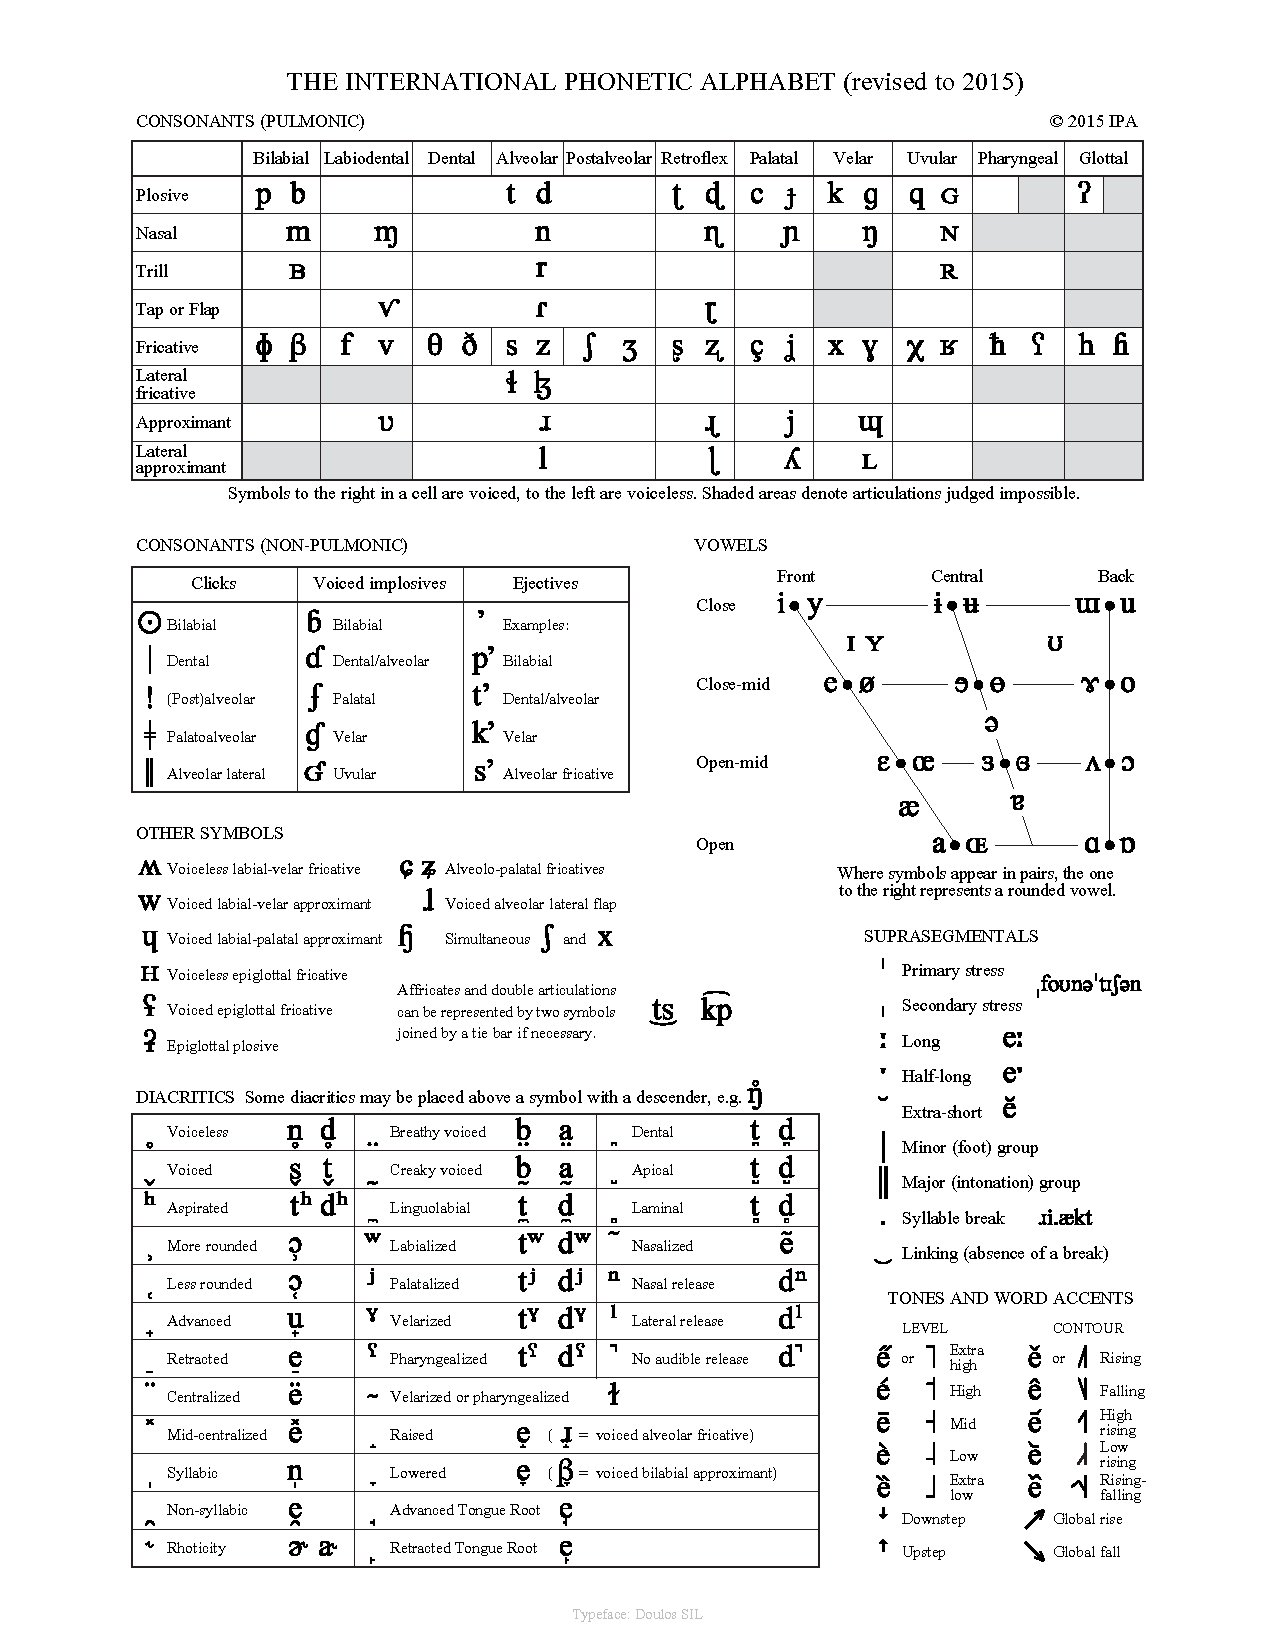
\includegraphics[scale=0.62]{ipaChart}}
    \caption{The International Phonetic Alphabet as defined by the International
    Phonetic Association}
    \label{ipaChart}
  \end{figure}

\newpage
% \nocite{*}
\printbibliography

\end{document}
